\documentclass{beamer}

% Use metropolis theme
\usepackage[progressbar=foot]{theme/beamerthememetropolis}
\usepackage{minted}
\usepackage{hyperref}

\title{Zarr vs. HDF5}

\date{November 4th, 2019}
\author{Joe Jevnik}
\institute{PyData NYC 2019}

\begin{document}
\maketitle

\newcommand{\zarr}{\texttt{zarr}}

\section{Core Concepts}

\begin{frame}{Multidimensional Data}
  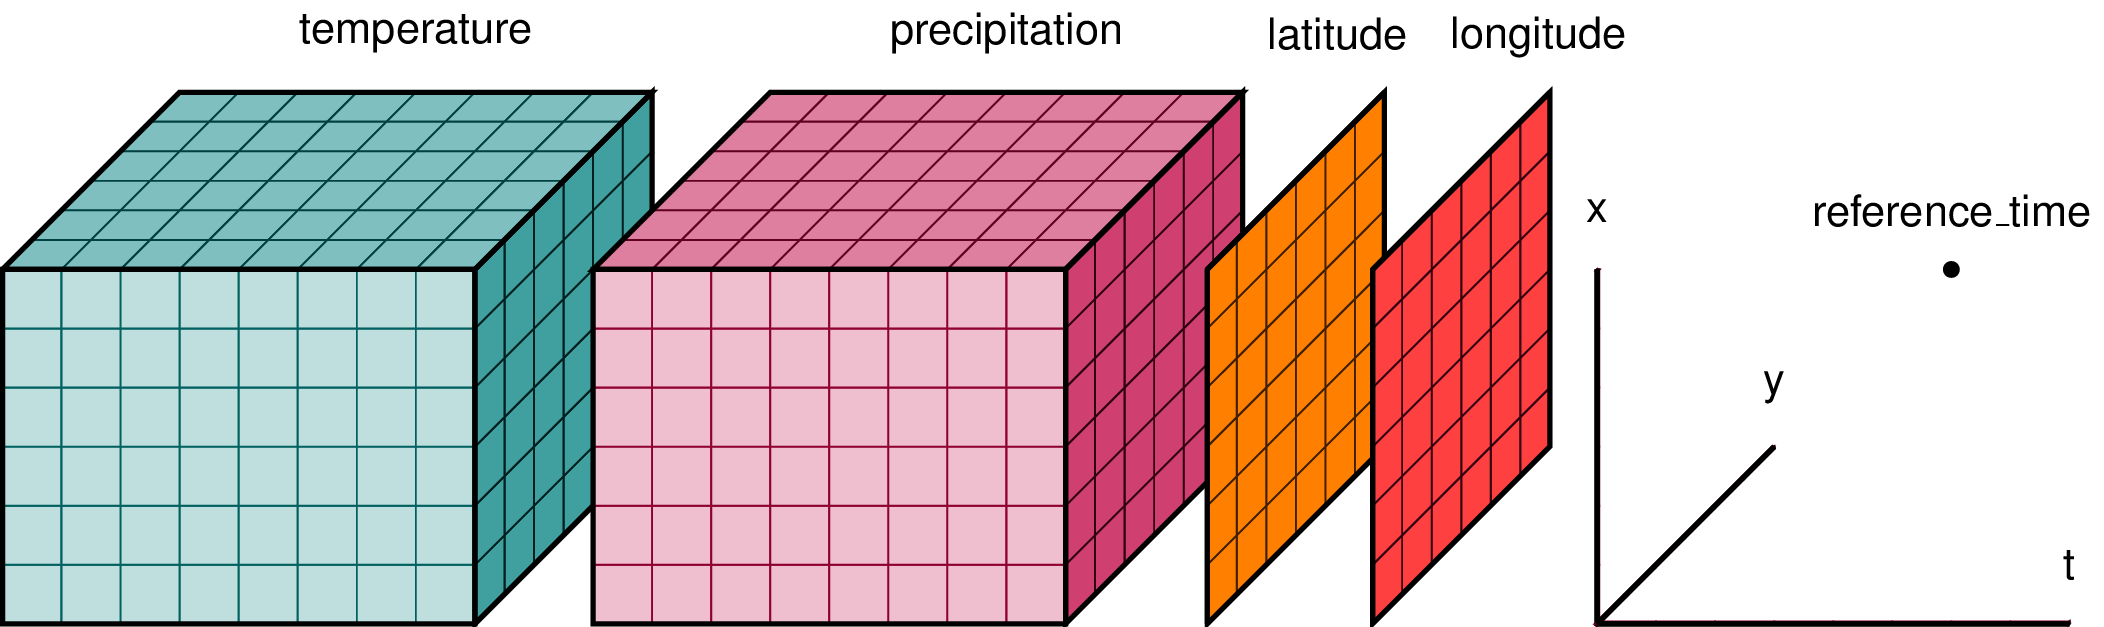
\includegraphics[width=1.00\textwidth]{images/multidimensional-data.png}
\end{frame}

\begin{frame}{Compression}
  \begin{itemize}
  \item[]<+-> same information in less space
  \item[]<+-> lossless
  \item[]<+-> lossy
  \end{itemize}
\end{frame}

\begin{frame}{Chunks}
  \begin{columns}[c]
    \column{0.5\textwidth}
    \begin{center}
      
\includegraphics[width=0.8\textwidth]{images/contig-data.png}
    \end{center}

    \column{0.5\textwidth}
    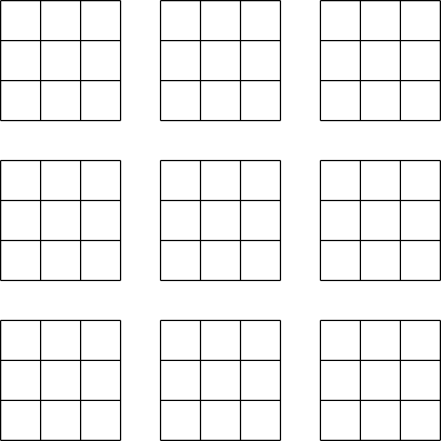
\includegraphics[width=0.8\textwidth]{images/block-chunks.png}
  \end{columns}
\end{frame}

\begin{frame}{Chunks}
  \begin{itemize}
  \item[]<+-> compression/random access trade off
  \item[]<+-> throughput/latency access trade off
  \item[]<+-> reduce io
  \item[]<+-> facilitate caching
  \end{itemize}
\end{frame}

\begin{frame}{Hierarchy}
  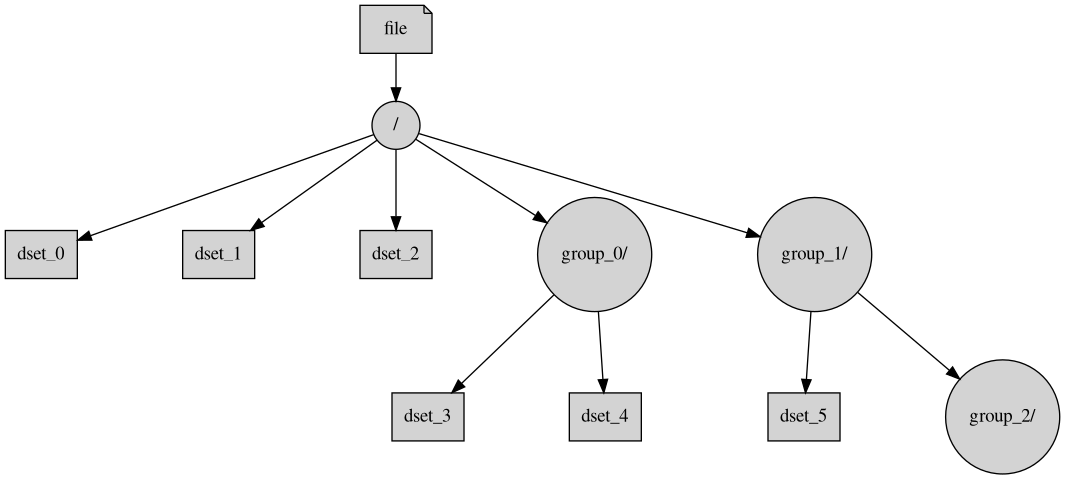
\includegraphics[width=1.0\textwidth]{images/tree.png}
\end{frame}

\begin{frame}{Nodes}
  \begin{definition}[Dataset]
    \begin{itemize}
    \item[] a multidimensional array
    \item[] leaves of a Zarr or HDF5 tree
    \end{itemize}
  \end{definition}
  \pause

  \begin{definition}[Group]
    \begin{itemize}
    \item[] collection of \textbf{datasets} or \textbf{groups}
    \end{itemize}
  \end{definition}
  \pause

  \begin{definition}[Node]
    \begin{itemize}
    \item[] either a \textbf{dataset} or \textbf{group}
    \end{itemize}
  \end{definition}
\end{frame}

\begin{frame}{Attributes}
  \begin{definition}[Attributes]
    \begin{itemize}
    \item[]<+-> key-value data
    \item[]<+-> property of each \textbf{node}
    \end{itemize}
  \end{definition}
\end{frame}

\section{Python Interface}

\begin{frame}{General}
  \begin{itemize}
  \item[]<+-> nested dictionaries
  \item[]<+-> leaves are \textit{array-like}
  \item[]<+-> supports numpy-style indexing
  \item[]<+-> NOTE: describes \texttt{h5py}, not \texttt{pytables}
  \end{itemize}
\end{frame}

\begin{frame}[fragile]{\zarr}
  \begin{minted}{python}
>>> import zarr
>>> f = zarr.open('file.zarr')
>>> f
<zarr.hierarchy.Group '/'>
  \end{minted}
  \pause

  \begin{minted}{python}
>>> f['dset'] = np.arange(20 * 5).reshape(20, 5)
>>> f['dset']
>>> <zarr.core.Array '/dset' (20, 5) int64>
\end{minted}
  \pause

  \begin{minted}{python}
>>> f['dset'][10, 3]
53
>>> f['dset'][:]
array([...]])
  \end{minted}
\end{frame}

\begin{frame}[fragile]{\texttt{h5py}}
  \begin{minted}{python}
>>> import h5py
>>> f = h5py.File('file.h5', 'r+')
>>> f
<HDF5 file "file.h5" (mode r+)>
  \end{minted}

  \begin{minted}{python}
>>> f['dset'] = np.arange(20 * 5).reshape(20, 5)
>>> f['dset']
<HDF5 dataset "dset": shape (20, 5), type "<i8">
\end{minted}

  \begin{minted}{python}
>>> f['dset'][10, 3]
53
>>> f['dset'][:]
array([...]])
  \end{minted}
\end{frame}

\begin{frame}{Extra Functionality}
  \begin{itemize}
  \item[]<+-> \texttt{Node.attrs} to get access to attributes as dict-like object
  \item[]<+-> \texttt{Group.create\_dataset} to set chunk shape and compression
  \item[]<+-> \texttt{Group.create\_group} to create sub-groups
  \item[]<+-> \texttt{Dataset.read\_direct} to read into existing buffers
  \end{itemize}
\end{frame}

\section{Making a Decision}

\begin{frame}{HDF5}
  \begin{itemize}
  \item<+-> over 20 years old
  \item<+-> excellent cross language support
  \item<+-> lots of existing software
  \item<+-> written in (very clean) C
  \item<+-> can be made thread safe, not thread optimal
  \item<+-> extensible in C
  \end{itemize}
\end{frame}

\begin{frame}{Zarr}
  \begin{itemize}
  \item<+-> first release in 2015, 1.0 on May 17, 2016
  \item<+-> written in Python, Python oriented
  \item<+-> has specification which could be reimplemented
  \item<+-> multithreading support
  \item<+-> extensible in Python
  \end{itemize}
\end{frame}

\begin{frame}{Extensions}
  \begin{itemize}
  \item[]<+-> filters and compressors
  \item[]<+-> storage backends
  \item[]<+-> which extensions come as part of the library itself?
  \item[]<+-> how to extend the libraries for non-default use cases?
  \item[]<+-> ease of distributing extensions
  \end{itemize}
\end{frame}

\section{Filters}

\begin{frame}{Filters}
  \begin{definition}[Filter]
    \begin{itemize}
    \item[]<+-> a function that sits between the raw data and the storage
    \item[]<+-> compressors
    \item[]<+-> checksumming
    \item[]<+-> composable
    \item[]<+-> act on one chunk at a time
    \end{itemize}
  \end{definition}
\end{frame}
      
\begin{frame}{Filters}
  \begin{columns}
    \column{0.5\textwidth}
    \begin{block}{write}
      \begin{center}
        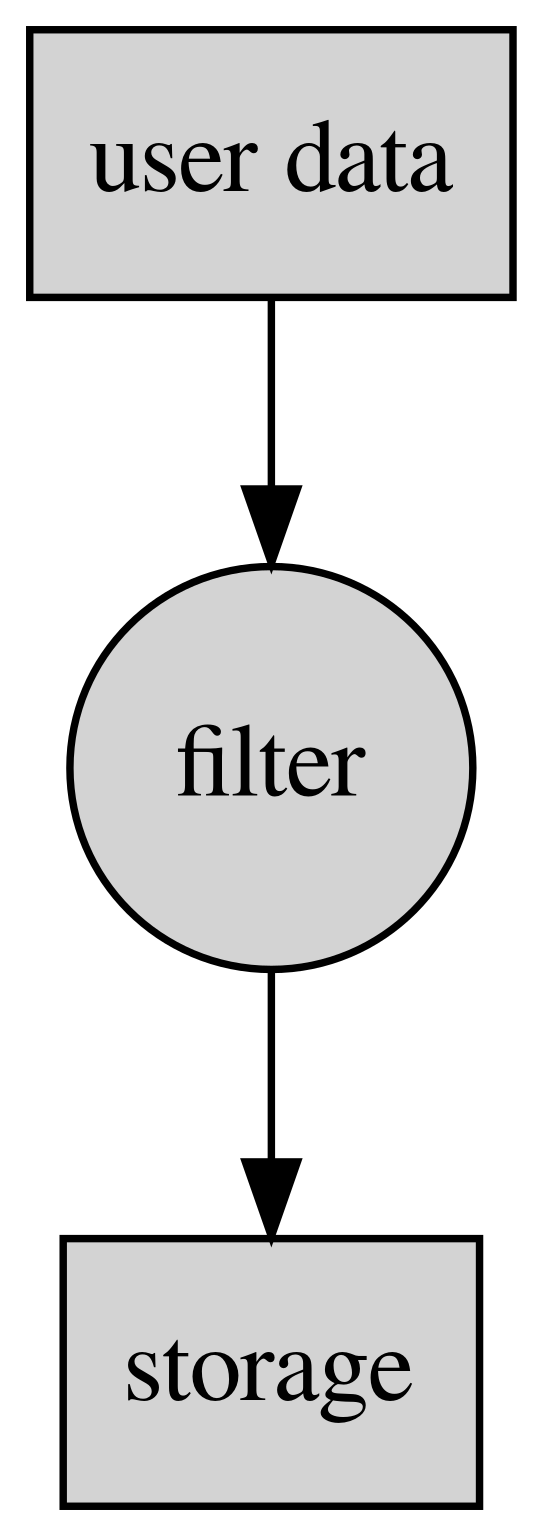
\includegraphics[height=0.75\textheight]{images/write-filter.png}
      \end{center}
    \end{block}

    \column{0.5\textwidth}
    \begin{block}{read}
      \begin{center}
        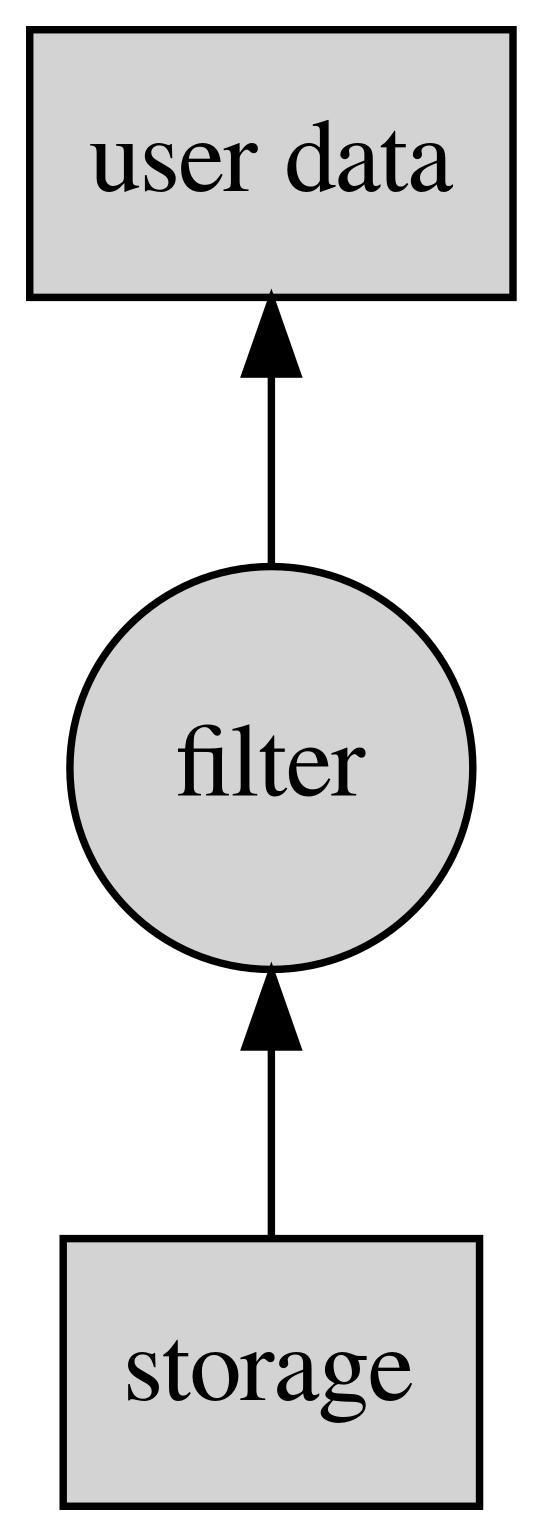
\includegraphics[height=0.75\textheight]{images/read-filter.png}
      \end{center}
    \end{block}
  \end{columns}
\end{frame}

\begin{frame}{Filter Pipelines}
  \begin{columns}
    \column{0.5\textwidth}
    \begin{block}{write}
      \begin{center}
        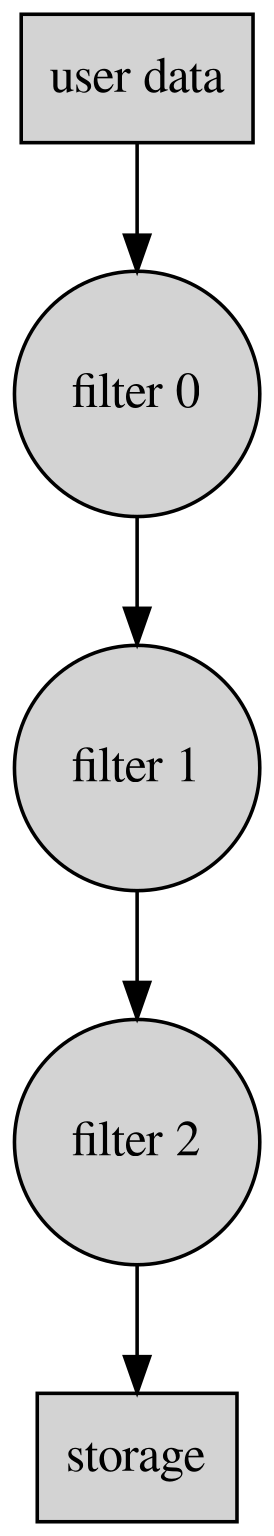
\includegraphics[height=0.75\textheight]{images/write-filter-pipeline.png}
      \end{center}
    \end{block}

    \column{0.5\textwidth}
    \begin{block}{read}
      \begin{center}
        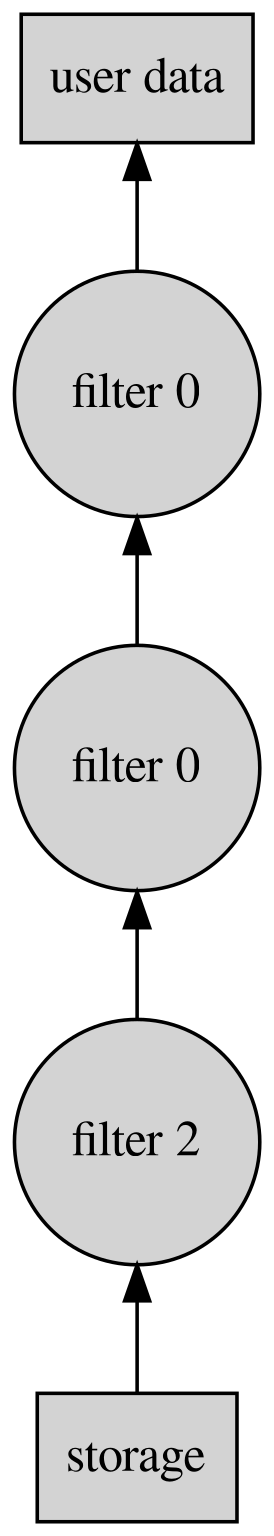
\includegraphics[height=0.75\textheight]{images/read-filter-pipeline.png}
      \end{center}
    \end{block}
  \end{columns}
\end{frame}

\begin{frame}{Default Filters in HDF5}
  \begin{itemize}
  \item \texttt{lzf}
  \item \texttt{gzip}
  \item \texttt{szip} (patent issues)
  \item \texttt{scale-offset} (lossy)
  \item \texttt{shuffle}
  \item \texttt{fletcher32} (checksum)
  \end{itemize}
\end{frame}

\begin{frame}{Default Filters in Zarr}
  \begin{columns}
    \column{0.5\textwidth}
    \begin{itemize}
    \item \texttt{blosc}
    \item \texttt{lz4}
    \item \texttt{zstd}
    \item \texttt{zlib}
    \item \texttt{gzip}
    \item \texttt{bz2}
    \item \texttt{lzma}
    \end{itemize}

    \column{0.5\textwidth}
    \begin{itemize}
    \item \texttt{delta}
    \item \texttt{fixed\_scale\_offset}
    \item \texttt{quantize} (lossy)
    \item \texttt{pack\_bits} (boolean packing)
    \item \texttt{categorical} (\texttt{str} $\rightarrow$ \texttt{int})
    \item \texttt{json}, \texttt{msgpack}, \texttt{pickle}
    \item \texttt{vlen\_string}
    \end{itemize}
  \end{columns}
\end{frame}

\begin{frame}[fragile]{Writing an HDF5 Filter}
  \begin{onslide}<1->
    \begin{minted}{c}
static size_t
f(unsigned int flags,
  size_t cd_nelmts, const unsigned cd_values[],
  size_t nbytes, size_t *buf_size, void **buf) {
    \end{minted}
  \end{onslide}
  \begin{onslide}<2->
    \begin{minted}{c}
    if (!(flags & H5Z_FLAG_REVERSE)) {
        /* encode data */
    }
    else {
        /* decode data */
    }
      \end{minted}
  \end{onslide}
  \begin{onslide}<3->
      \begin{minted}{c}
    return /* number of bytes in new buffer
              or 0 on failure */;
    \end{minted}
  \end{onslide}
  \begin{onslide}<1->
    \begin{minted}{c}
}
    \end{minted}
  \end{onslide}  
\end{frame}

\begin{frame}[fragile]{Writing an HDF5 Filter Cont.}
  \begin{minted}{c}
static htri_t
can_apply(hid_t dcpl_id, hid_t type_id, hid_t space_id) {
    /* return -1 for error, 0 for false, or 1 for true */
}
  \end{minted}
\end{frame}

\begin{frame}[fragile]{Writing an HDF5 Filter Cont.}
  \begin{minted}{c}
const int my_filter_id = /* ... */;
static H5Z_class2_t filter = {
    .version = H5Z_CLASS_T_VERS,
    .id = my_filter_id,
    .encoder_present = 1,
    .decoder_present = 1,
    .name = "my_filter",
    .can_apply = can_apply,
    .set_local = NULL,
    .filter = f,
};

int my_filter_register() { return H5Zregister(&filter); }
  \end{minted}
\end{frame}

\begin{frame}[fragile]{Using a Custom HDF5 Filter}
\begin{minted}{python}
import ctypes
dll = ctypes.CDLL('filter.so')
assert dll.my_filter_register() == 0
filter_id = ctypes.c_int.in_dll(
    dll, 'my_filter_id',
).value
  \end{minted}
  \pause

  \begin{minted}{python}
f = h5py.File('a.h5', 'r+')
dset = f.create_dataset(
    'dset',
    compression=filter_id,
    dtype='i8',
    shape=(100,),
)
  \end{minted}
\end{frame}

\begin{frame}{Difficulties with Custom HDF5 Filters}
  \begin{itemize}
  \item[]<+-> \texttt{h5py} statically links to \texttt{hdf5} by default
  \item[]<+-> \texttt{h5py} doesn't re-export \texttt{H5Zregister}
  \item[]<+-> \texttt{\$ HDF5\_VERSION=1.10 pip install --no-binary :all: h5py}
  \item[]<+-> hard to thread parameters
  \item[]<+-> hard to manage state
  \item[]<+-> must use \texttt{malloc}/\texttt{free}
  \item[]<+-> can't use custom pipelines in \texttt{h5py} yet (I think)
  \item[]<+-> doesn't trigger until flush
  \end{itemize}
\end{frame}

\begin{frame}{Good Points with Custom HDF5 Filters}
  \begin{itemize}
  \item[]<+-> filter ids use central authority
  \item[]<+-> can be used in different languages
  \item[]<+-> plugin directory to find extension
  \end{itemize}
\end{frame}

\begin{frame}[fragile]{Writing a Zarr Filter}
  \begin{minted}{python}
import numcodecs
from numcodecs.abc import Codec

class MyFilter(Codec):
    codec_id = 'my_filter'

    def encode(self, buf):
        ...

    def decode(self, buf, out=None):
        ...

numcodecs.register_codec(MyFilter)
  \end{minted}
\end{frame}

\begin{frame}[fragile]{Using a Custom Zarr Filter}
  \begin{minted}{python}
import numpy as np
import zarr

from my_filter import MyFilter

f = zarr.open('a.zarr', 'w')
dset = f.create_dataset(
    'dset',
    compressor=MyFilter(),
    #filters=[..., MyFilter(), ...],
    dtype='i8',
    shape=(100,),
)
  \end{minted}
\end{frame}

\begin{frame}{Problems with Custom Zarr Filters}
  \begin{itemize}
  \item[]<+-> no central authority, names can collide
  \item[]<+-> require Python code or an alternative implementation
  \item[]<+-> probably want to be written in native code anyways
  \end{itemize}
\end{frame}

\begin{frame}{Good Points with Custom Zarr Filters}
  \begin{itemize}
  \item[]<+-> written in Python
  \item[]<+-> easy distribution (Python package)
  \item[]<+-> easy to pass parameters to filter
  \item[]<+-> easy to manage state
  \item[]<+-> split API is more clear
  \item[]<+-> easily works in filter pipelines
  \end{itemize}
\end{frame}

\begin{frame}{Delta of Deltas Example}
  \url{https://github.com/llllllllll/zarr-vs-hdf5-talk/blob/master/examples/delta_of_delta_filter}
\end{frame}

\section{Storage}

\begin{frame}{Storage Protocol}
  \begin{itemize}
  \item[]<+-> abstract storage of structures
  \item[]<+-> no single file type
  \item[]<+-> configurable
  \item[]<+-> two kinds of data
  \item[]<+-> user data
  \item[]<+-> metadata (tree structure, extra driver info)
  \end{itemize}
\end{frame}

\begin{frame}{HDF5 Storage Model}
  \begin{itemize}
  \item[]<+-> virtual contiguous memory space
  \item[]<+-> allocator-like
  \item[]<+-> no information about semantic data
  \item[]<+-> library handles caching/locking
  \item[]<+-> single threaded
  \end{itemize}
\end{frame}

\begin{frame}{Zarr Storage Model}
  \begin{itemize}
  \item[]<+-> based on \texttt{dict} from \texttt{str} to \texttt{bytes}
  \item[]<+-> Python mapping protocol
  \item[]<+-> key contains semantic information
  \item[]<+-> \texttt{group/dset/0.3}
  \item[]<+-> can manage locking, not required
  \item[]<+-> composable
  \end{itemize}
\end{frame}

\begin{frame}{Default Storage Backends in HDF5}
  \begin{itemize}
  \item<+-> \texttt{sec2} (posix API)
  \item<+-> \texttt{windows} (Windows file API)
  \item<+-> \texttt{stdio} (buffered, C \texttt{stdio.h})
  \item<+-> \texttt{core} (in memory)
  \item<+-> \texttt{family} (directory of blocks)
  \item<+-> \texttt{fileobj} (\texttt{h5py} only)
  \end{itemize}
\end{frame}

\begin{frame}{Default Storage Backends in Zarr}
  \begin{columns}
    \column{0.45\textwidth}
    \begin{itemize}
    \item \texttt{MemoryStore}
    \item \texttt{DirectoryStore}
    \item \texttt{TempStore}
    \item \texttt{NestedDirectoryStore}
    \item \texttt{ZipStore} (single file)
    \item \texttt{DBMStore}
    \item \texttt{LMDBStore}
    \end{itemize}

    \column{0.55\textwidth}
    \begin{itemize}
    \item \texttt{SQLiteStore}
    \item \texttt{MongoDBStore}
    \item \texttt{RedisStore}
    \item \texttt{ABSStore} (Azure Blob Storage)
    \item \texttt{LRUStoreCache}
    \item \texttt{ConsolidatedMetadataStore}
    \item \texttt{S3Map} (third party)
    \end{itemize}
  \end{columns}
\end{frame}

\begin{frame}[fragile]{Writing a Custom HDF5 File Driver}
  \begin{minted}{c}
struct H5FD_class_t;
  \end{minted}
  \pause
  
  \begin{minted}{c}
herr_t (*write)(H5FD_t* file, H5FD_mem_t type,
                hid_t dxpl, haddr_t addr,
                size_t size, const void* buffer);
  \end{minted}
  \pause

  \begin{minted}{c}
herr_t (*read)(H5FD_t* file, H5FD_mem_t type,
               hid_t dxpl, haddr_t addr,
               size_t size, void* buffer);
  \end{minted}
  \pause

  \begin{minted}{c}
/* 28 more member functions and
   static member variables */
  \end{minted}

\end{frame}

\begin{frame}[fragile]{Using a Custom HDF5 File Driver}
  \begin{minted}{python}
    import h5py

    from my_driver_as_extension_module import set_fapl

    h5py.register_driver('my_driver', set_fapl)
  \end{minted}
  \pause

  \begin{minted}{python}
    file = h5py.File(
        'path/to/pass/to/driver/open'
        'w',
        driver='my_driver',
        **extra_driver_kwargs,
    )
  \end{minted}
\end{frame}

\begin{frame}{Problems with Custom HDF5 File Drivers}
  \begin{itemize}
  \item[]<+-> huge API
  \item[]<+-> no semantic information
  \item[]<+-> hard to optimize
  \item[]<+-> not composable
  \item[]<+-> need to rely on HDF5 to do a lot of things for you
  \item[]<+-> small ABI incompatibility between 1.8 and 1.10
  \item[]<+-> single threaded
  \item[]<+-> not many people have published file drivers
  \end{itemize}
\end{frame}

\begin{frame}{Good Points with Custom HDF5 File Drivers}
  \begin{itemize}
  \item[]<+-> \texttt{set\_fapl} makes it easy to thread arguments
  \item[]<+-> reasonable state management
  \item[]<+-> source code of built in drivers is very clear
  \item[]<+-> can be built to minimize copies
  \item[]<+-> can flatten or cut up the data to use different drivers
  \item[]<+-> 64 bit memory space always
  \end{itemize}
\end{frame}

\begin{frame}[fragile]{Writing a Custom Zarr Storage Backend}
  \begin{minted}{python}
from collections.abc import MutableMapping

class MyStorageBackend(MutableMapping):
    def __getitem__(self, key):
        ...

    def __setitem__(self, key, data):
        ...

    def __delitem__(self, key):
        ...

    # ... __iter__, __len__
  \end{minted}
\end{frame}

\begin{frame}{Problems with Custom Zarr Storage Backends}
  \begin{itemize}
  \item[]<+-> always need to copy on read
  \end{itemize}
\end{frame}

\begin{frame}{Good Points with Custom Zarr Storage Backends}
  \begin{itemize}
  \item[]<+-> composable
  \item[]<+-> user defined caching, consolidation, etc.
  \item[]<+-> semantic information available
  \item[]<+-> written in Python
  \end{itemize}
\end{frame}

\section{Conclusion}

\begin{frame}{Takeaways}
  \begin{columns}
    \column{0.50\textwidth}
    \begin{block}{Zarr}
      \begin{itemize}
      \item lots of modern features
      \item actively developed
      \item responsive and helpful devs
      \item Python focused/specific*
      \item easier to prototype extensions
      \end{itemize}
    \end{block}

    \column{0.50\textwidth}
    \begin{block}{HDF5}
      \begin{itemize}
      \item stable mature code
      \item cross language support
      \item very single threaded
      \item harder to write extensions
      \end{itemize}
    \end{block}
  \end{columns}
\end{frame}

\begin{frame}{Thank You}
  \begin{itemize}
  \item \url{https://github.com/llllllllll} (10 lowercase L's)
  \item Example delta of deltas filter for both HDF5 and Zarr:
    \url{https://github.com/llllllllll/zarr-vs-hdf5-talk/blob/master/examples/delta_of_delta_filter}
  \item S3 file driver for HDF5: \url{https://github.com/h5s3/h5s3}
  \item \texttt{@\_\_qualname\_\_}
  \end{itemize}
\end{frame}

\end{document}